\hsection{Python in the Terminal}%
\label{sec:pythonInTheTerminal}%
\FloatBarrier%
%
\begin{figure}%
\centering%
%
\subfloat[][%
Open a \pgls{terminal} (by pressing \ubuntuTerminal\ under \ubuntu\ \linux; under \windows\ \windowsTerminal). %
Change into the directory \inQuotes{directory} where your \python\ file is located, by typing \bashil{cd directory} and hit \keys{\enter}.%
\label{fig:terminalPython1cd}%
]{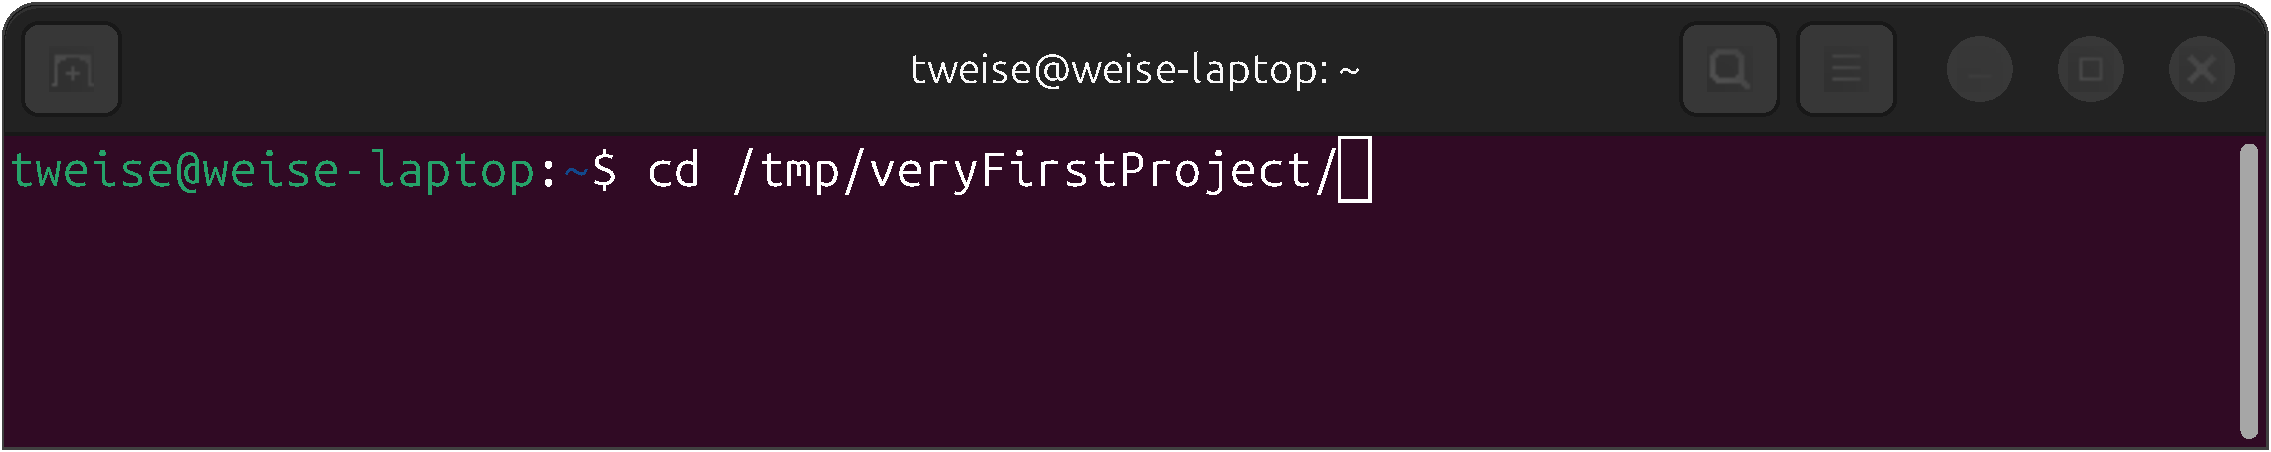
\includegraphics[width=0.9\linewidth]{\currentDir/terminalPython1cd}}%
%
\floatRowSep%
%
\subfloat[][%
Execute a \python\ program \inQuotes{program.py} by typing \bashil{python3 program.py} and hit \keys{\enter}. %
In our case, the program is \inQuotes{very\_first\_program.py}.%
\label{fig:terminalPython2python}%
]{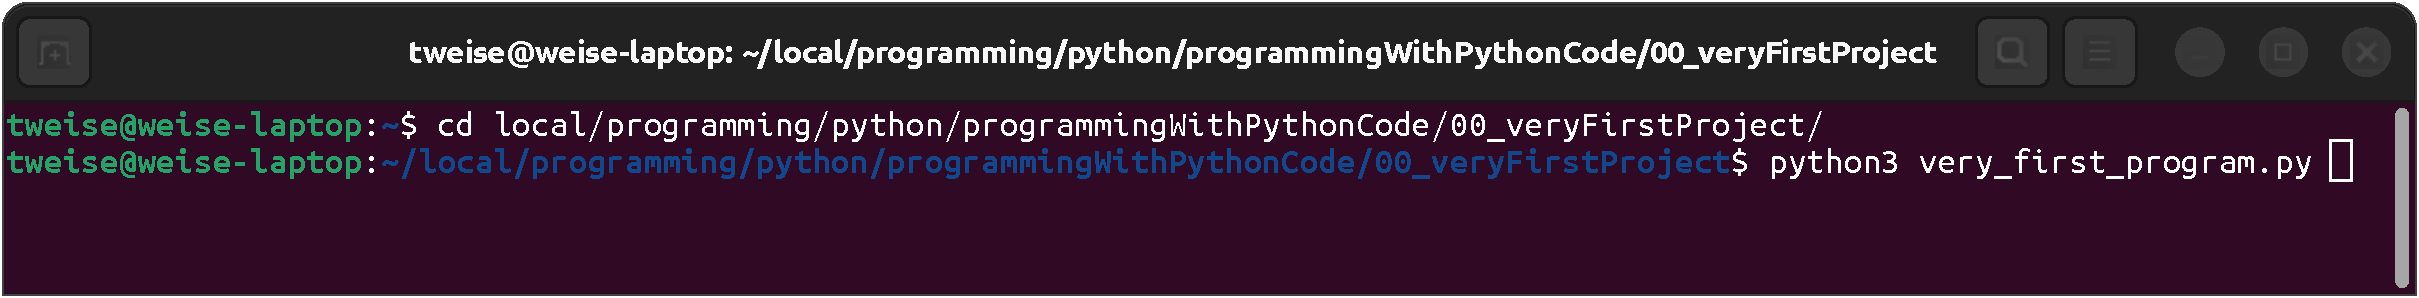
\includegraphics[width=0.9\linewidth]{\currentDir/terminalPython2python}}%
%
\floatRowSep%
%
\subfloat[][%
As expected, the text \inQuotes{Hello World!} appears in the \pgls{terminal}.%
\label{fig:terminalPython3result}%
]{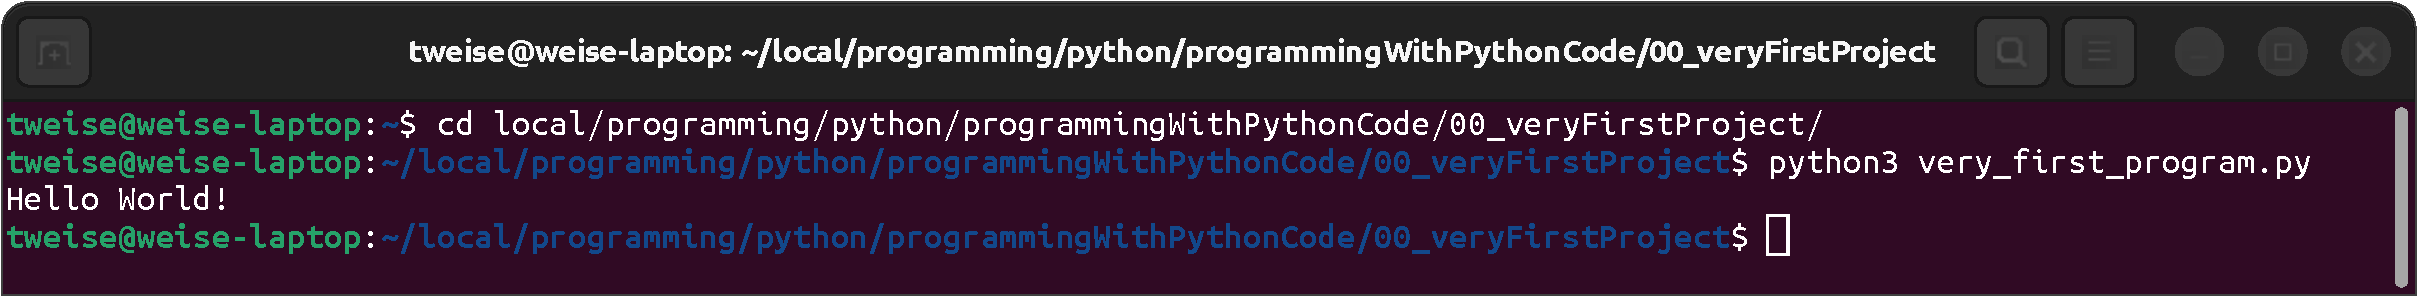
\includegraphics[width=0.9\linewidth]{\currentDir/terminalPython3result}}%
%
\caption{Example of executing a \python\ program in a \pgls{terminal} (on \ubuntu).}%
\label{fig:terminalPython}%
\end{figure}%
%
\begin{figure}%
\centering%
%
\subfloat[][%
Pressing the \menu{\pycharmConsole} on the vertical icon bar on the left side of the \pycharm\ window.%
\label{fig:pycharmConsole1consoleButton}%
]{\tightbox{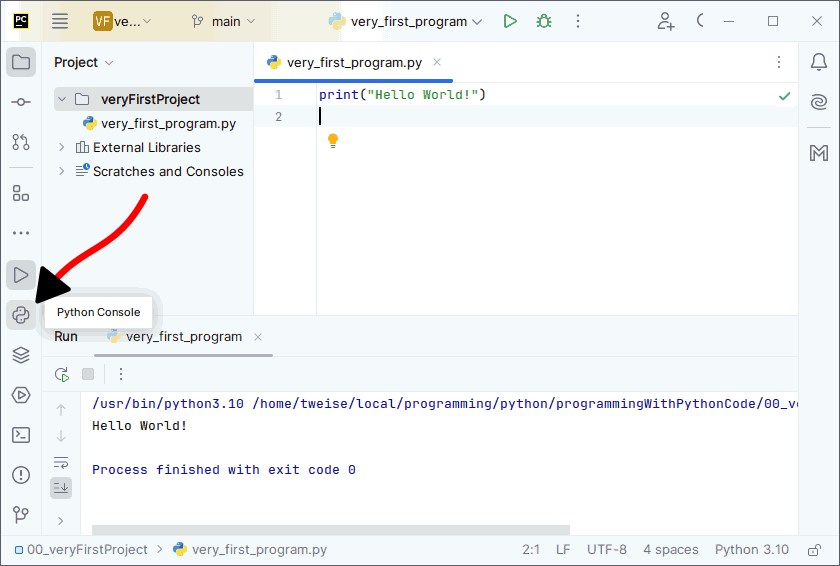
\includegraphics[width=0.76\linewidth]{\currentDir/pycharmConsole1consoleButton}}}%
%
\floatRowSep%
%
\subfloat[][%
The \pycharm\ \python\ console is open.%
\label{fig:pycharmConsole2consoleOpen}%
]{\tightbox{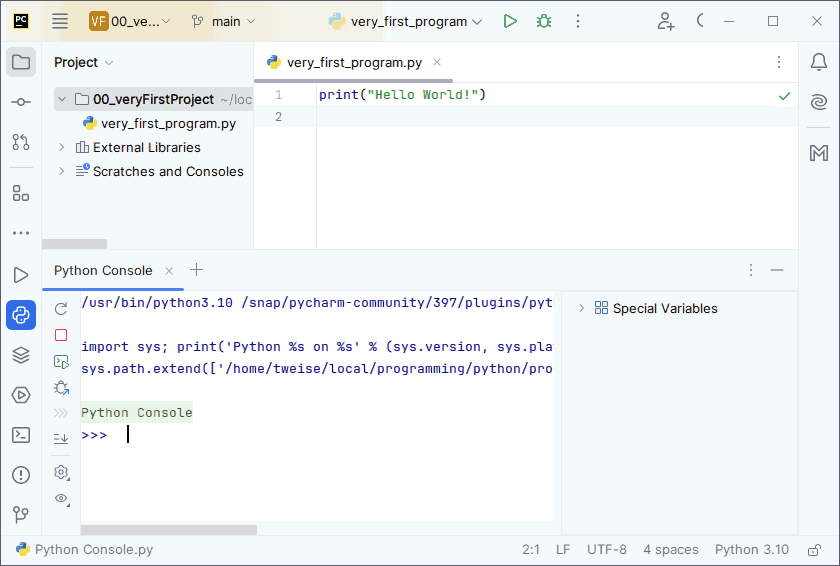
\includegraphics[width=0.76\linewidth]{\currentDir/pycharmConsole2consoleOpen}}}%
%
\caption{Entering the \inQuotes{Hello World!} program from \cref{lst:very_first_program} directly into the \python\ console offered by \pycharm.}%
\label{fig:pycharmConsoleA}%
\end{figure}%
\begin{figure}%
\ContinuedFloat%
\centering%
%
\subfloat[][%
We enter the \inQuotes{Hello World!} program from \cref{lst:very_first_program} and press \keys{\enter}.%
\label{fig:pycharmConsole3writingCode}%
]{\tightbox{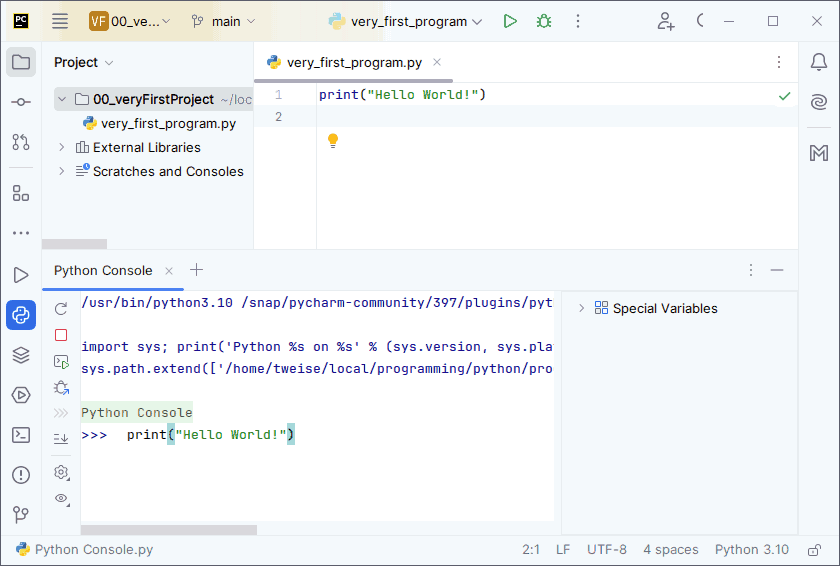
\includegraphics[width=0.76\linewidth]{\currentDir/pycharmConsole3writingCode}}}%
%
\floatRowSep%
%
\subfloat[][%
And indeed, the output is \inQuotes{Hello World!}.%
\label{fig:pycharmConsole4codeOutput}%
]{\tightbox{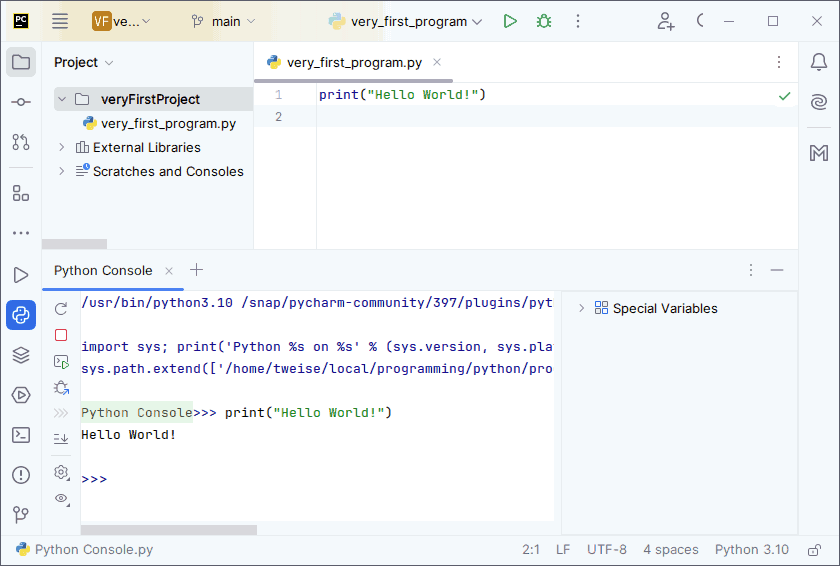
\includegraphics[width=0.76\linewidth]{\currentDir/pycharmConsole4codeOutput}}}%
%
\caption{Entering the \inQuotes{Hello World!} program from \cref{lst:very_first_program} directly into the \python\ console offered by \pycharm~(continued).}%
\label{fig:pycharmConsoleB}%
\end{figure}%
%
\begin{figure}%
\centering%
%
\subfloat[][%
Open a \pgls{terminal} (by pressing \ubuntuTerminal\ under \ubuntu\ \linux; under \windows\ \windowsTerminal), enter \bashil{python3}, then hit \keys{\enter}.%
\label{fig:terminalConsole1python}%
]{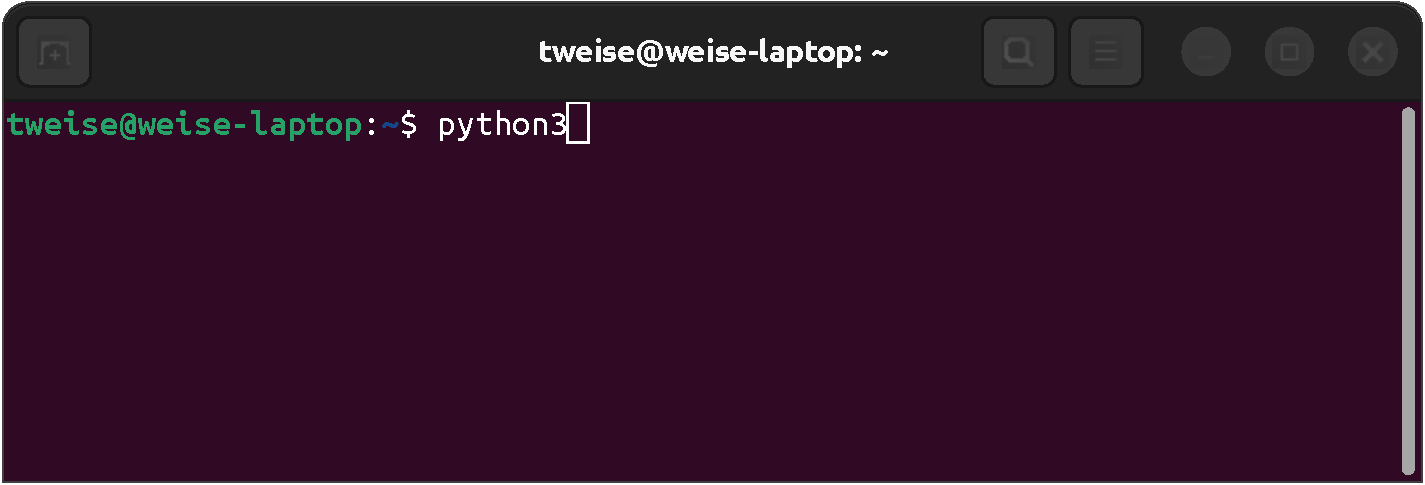
\includegraphics[width=0.852\linewidth]{\currentDir/terminalConsole1python}}%
%
\floatRowSep%
%
\subfloat[][%
The \python\ console opens in the \pgls{terminal}.%
\label{fig:terminalConsole2pythonRunning}%
]{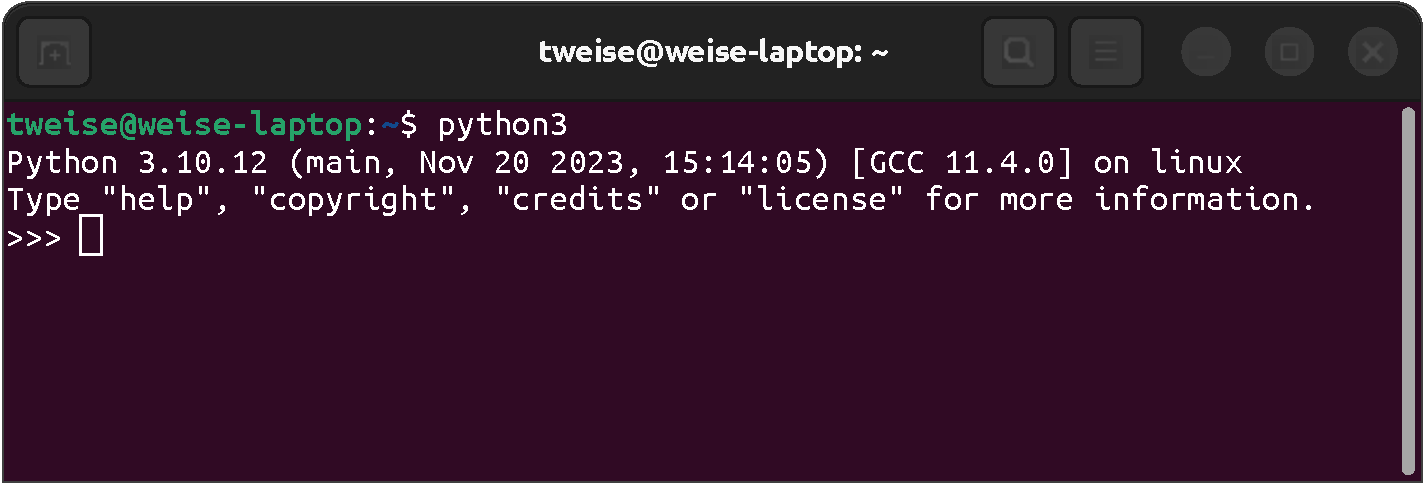
\includegraphics[width=0.852\linewidth]{\currentDir/terminalConsole2pythonRunning}}%
%
\floatRowSep%
%
\subfloat[][%
We enter the \inQuotes{Hello World!} program from \cref{lst:very_first_program} and press \keys{\enter}.%
\label{fig:terminalConsole3writingCode}%
]{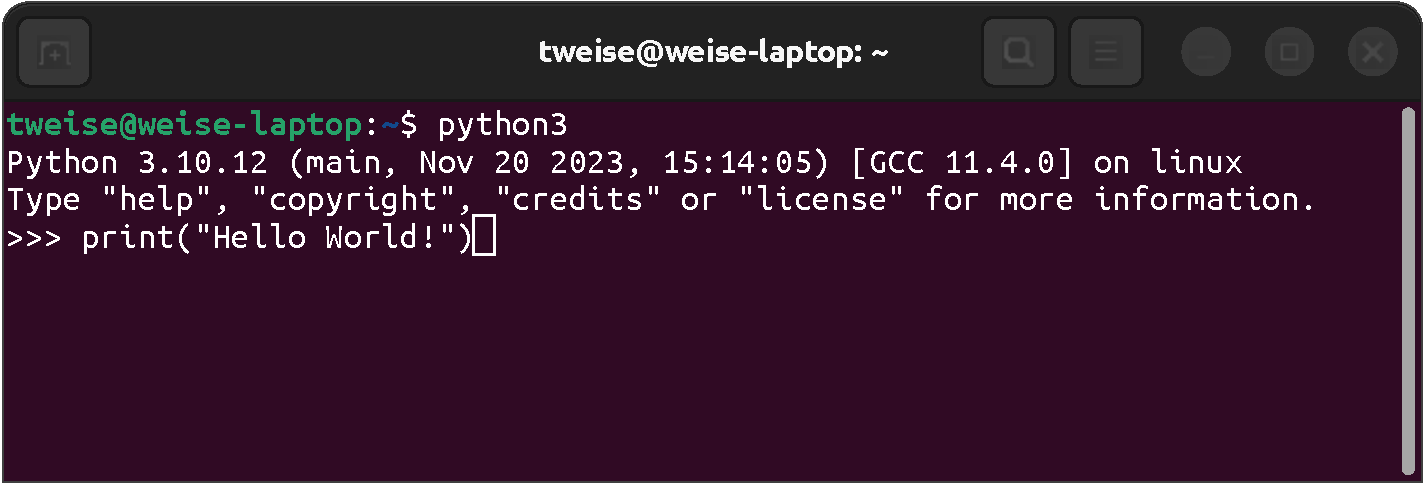
\includegraphics[width=0.852\linewidth]{\currentDir/terminalConsole3writingCode}}%
%
\floatRowSep%
%
\subfloat[][%
And indeed, the output is \inQuotes{Hello World!}.%
\label{fig:terminalConsole4codeOutput}%
]{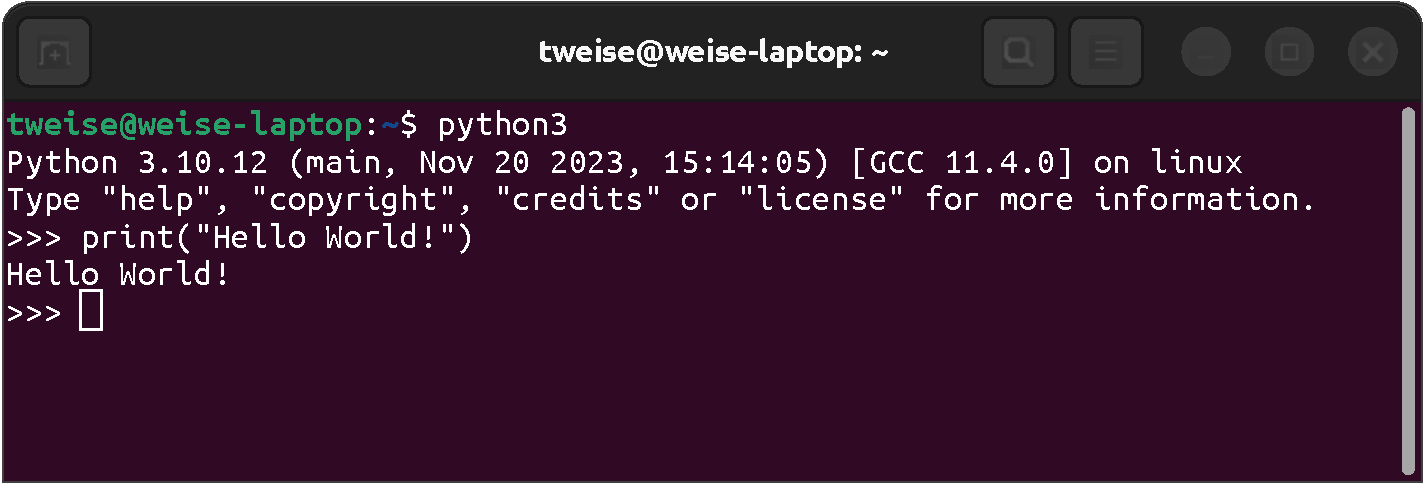
\includegraphics[width=0.852\linewidth]{\currentDir/terminalConsole4codeOutput}}%
%
\caption{Writing a program in the \python\ console in the \pgls{terminal}~(\ubuntu).}%
\label{fig:terminalConsoleA}%
\end{figure}%
\begin{figure}%
\ContinuedFloat%
\centering%
%
\subfloat[][%
We exit the console by typing \pythonil{exit()} and pressing \keys{\enter}.%
\label{fig:terminalConsole5exit}%
]{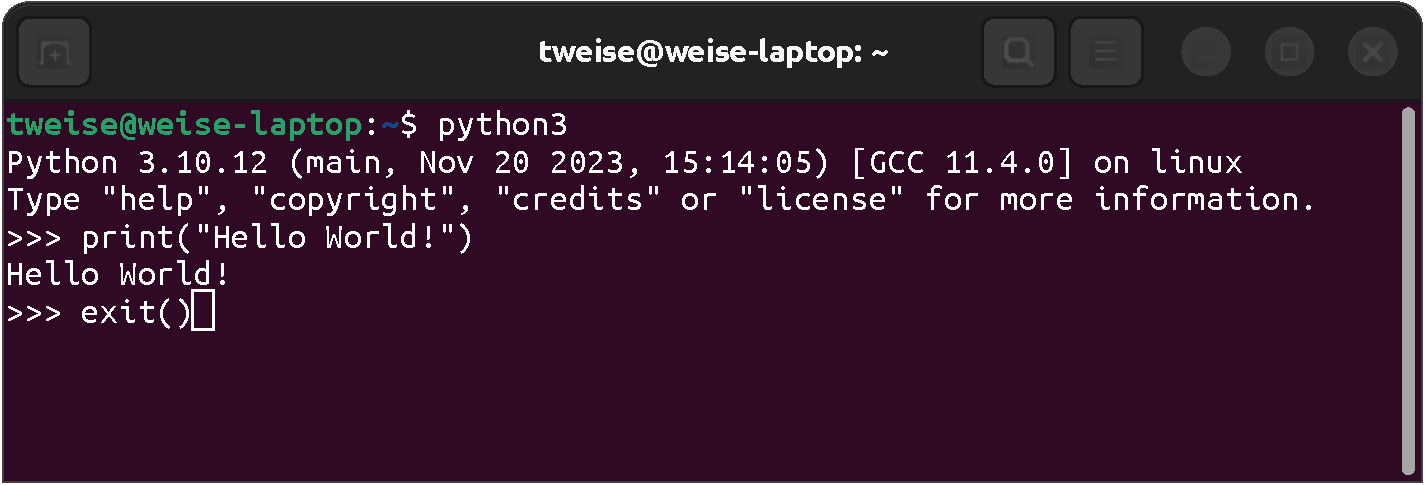
\includegraphics[width=0.852\linewidth]{\currentDir/terminalConsole5exit}}%
%
\floatRowSep%
%
\subfloat[][%
We are back in the normal \pgls{terminal}.%
\label{fig:terminalConsole6left}%
]{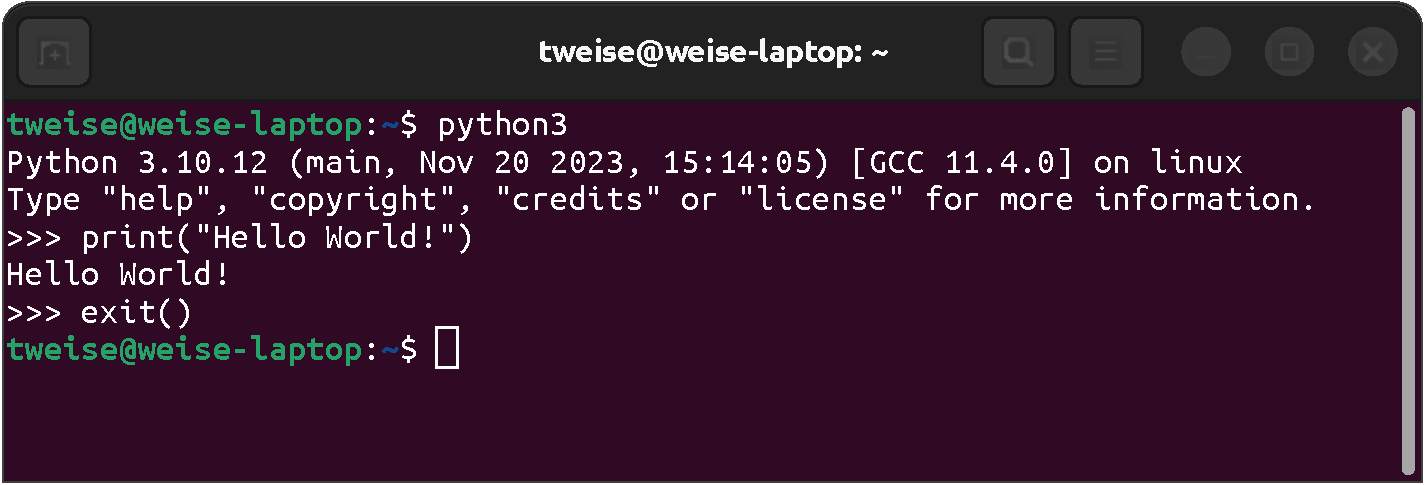
\includegraphics[width=0.852\linewidth]{\currentDir/terminalConsole6left}}%
%
\caption{Writing a program directly in the \python\ console in the \pgls{terminal}~(\ubuntu,~continued).}%
\label{fig:terminalConsoleB}%
\end{figure}%
%
In total, are four more ways in which we can execute a \python\ program:%
%
\begin{enumerate}%
%
\item We can enter the program into a \python\ file in the \pycharm\ \pgls{ide} and then run it from there. %
We just did this in the previous section and illustrated it in \cref{fig:veryFirstProgramC}.%
%
\item Actually, we can also write a \python\ program with a normal text editor. %
A \python\ program is just a normal text file, after all. %
We can execute such a text file by entering its directory and typing \bashil{python3 programName} (where \bashil{programName} is \bashil{very_first_program.py}, in our case) and hitting \keys{\enter}. %
Then the program is executed directly in the \pgls{terminal}. %
This process is shown in \cref{sec:terminalPython,fig:terminalPython}.%
%
\item Alternatively, we could open the \python\ interpreter console in \pycharm\ and enter and execute our code line-by-line. %
This is sketched in \cref{sec:pycharmConsole,fig:pycharmConsoleA}.%
%
\item Besides using the \python\ console inside \pycharm, we can also open it inside a \pgls{terminal}. %
We can then enter separate \python\ instructions and run them there. %
This fourth option is outlined in \cref{sec:terminalConsolem,fig:terminalConsoleA}.%
%
\end{enumerate}%
%
\hsection{Executing a \python\ Program in a Terminal}%
\label{sec:terminalPython}%
In order to directly execute a \python\ program in a \pgls{terminal}, we first need to open one.
Under \ubuntu\ \linux, we simply press \ubuntuTerminal.
Under \windows, we have to \windowsTerminal.
Once the terminal is open, we need to change into the directory where the program is located.
Under both \linux\ and \windows, this can be done by typing the command \bashil{cd}, followed by the path to the directory, and hitting \keys{\enter}.\footnote{%
Under \windows, you may also need to change into the correct drive first.}
We provide a screenshot for that, taken under \ubuntu\ \linux, in \cref{fig:terminalPython1cd}.
Now we simply call the \python\ interpreter by writing \bashil{python3} followed by the file name of our program, which is \bashil{very_first_program.py} in our case.
In \cref{fig:terminalPython2python} we do this and hit \keys{\enter}, which causes the \python\ interpreter to execute our program.
The output \inQuotes{Hello World!} is then printed into the \pgls{terminal} in \cref{fig:terminalPython3result}.%
\endhsection%
%
\hsection{Entering Commands in the \python\ Console inside \pycharm}%
\label{sec:pycharmConsole}%
Besides writing programs in files and executing them, we can also directly enter them into the \python\ console and execute them step-by-step.
This does not make sense if we want to reuse our programs later.
But it does make a lot of sense when we just want to test some commands or functions or quickly test some idea.
A \python\ console can be used directly in \pycharm~(\cref{fig:pycharmConsoleA}) or opened in a \pgls{terminal}~(\cref{fig:terminalConsoleA}).

To explore entering \python\ code in the \python\ console inside \pycharm, we continue where we left of in \cref{sec:ourFirstProgram}.
In \pycharm, we first click the \menu{\pycharmConsole} on the vertical icon bar on the left side of the \pycharm\ window, as shown in \cref{fig:pycharmConsole1consoleButton}.
This directly brings us to the \python\ console~(\cref{fig:pycharmConsole2consoleOpen}).
We can enter the one-line-program from \cref{lst:very_first_program}, as illustrated in \cref{fig:pycharmConsole3writingCode}.
Notice that the input prompt of the console is marked by the three greater characters \bashil{>>>} after which we enter our text.
Pressing \keys{\enter} after writing the code leads to the expected output shown in \cref{fig:pycharmConsole4codeOutput}.
This output directly appears in the console and is not preceded by any other text, in particular not by \bashil{>>>}, which makes it easy to visually distinguish what the input and output in a \python\ console are.%
\endhsection%
%
\hsection{Entering Commands in the \python\ Console in a Terminal}%
\label{sec:terminalConsolem}%
Let us now open a \python\ console from the \pgls{terminal} instead of using the one in \pycharm.
We therefore first need to open a normal terminal.
Under \ubuntu\ \linux, we simply press \ubuntuTerminal.
Under \windows, we have to \windowsTerminal.
Either way, the terminal opens and we can enter \bashil{python3} and press \keys{\enter}, as shown in \cref{fig:terminalConsole1python}.
Now the \python\ interpreter starts right inside the \pgls{terminal}~(\cref{fig:terminalConsole2pythonRunning}).
The prompt, i.e., the place where we can write our code, again is preceded by the \bashil{>>>} characters.
As illustrated in \cref{fig:terminalConsole3writingCode}, we copy the single line of code, \pythonil{print("Hello World!")}\pythonIdx{print} from \cref{lst:very_first_program} and press \keys{\enter}.
The output \inQuotes{Hello World!} is printed as expected in \cref{fig:terminalConsole4codeOutput}.
However, we now are still in the \python\ interpreter.
In order to leave it and to, maybe, enter other commands in the \pgls{terminal}, we have to use another new \python\ instruction:
We type in \pythonil{exit()} and press \keys{\enter}, as shown in \cref{fig:terminalConsole5exit}, which causes the \python\ interpreter to exit.
We are now back in the basic terminal, as shown in \cref{fig:terminalConsole6left}.
In these figures, I was using \ubuntu\ \linux.
On \windows\ or other \linux\ variants, the process would have looked quite similar.%
\endhsection%
%
\bestPractice{runningProgram}{The only proper way to run a \python\ application in a productive scenario is in the terminal, as shown in \cref{sec:terminalPython}.}%
\endhsection%
%
